\documentclass{ximera}

\begin{document}
	\author{Stitz-Zeager}
	\xmtitle{TITLE}


\mfpicnumber{1}

\opengraphsfile{TheLawofSines}

\setcounter{footnote}{0}

\label{TheLawofSines}

In this chapter, we showcase how the the tools we've developed in Chapters \ref{FoundationsofTrigonometry} and \ref{AnalyticalTrigonometry} can be applied to Geometry.  Our first two sections focus specifically on solving oblique (non-right) Triangles.\footnote{Recall that the word `Trigonometry' literally means `measuring triangles' so we are returning to our roots here.} 

\smallskip

Our first example reviews the basics of right triangle trigonometry.  The reader is referred to Section \ref{AppRightTrig} for more details and practice with these concepts.


\begin{example}  \label{righttrianglereviewex}  Given a right triangle with a hypotenuse of length $7$ units and one leg of length $4$ units, find the length of the remaining side and the measures of the remaining angles. Express the angles in decimal degrees, rounded to the nearest hundredth of a degree.

\smallskip

{\bf Solution.}  For definitiveness, we label the triangle below. 

\begin{center}

\begin{mfpic}[18]{0}{4}{0}{6}
\tlabel[cc](2,-1){$b=4$}
\tlabel(4.25,2){$a$}
\tlabel[cc](1.75,0.75){$\alpha$}
\tlabel[cc](3.25,3.5){$\beta$}
\arrow \reverse \arrow \parafcn{5, 50, 5}{1.5*dir(t)}
\arrow \reverse \arrow \shiftpath{(4,5.75)}  \parafcn{240, 265, 5}{1.5*dir(t)}
\tlpointsep{-10pt}
\tlabel(0,0){\rotatebox{55}{\hspace{.75in}$c = 7$}}
\polyline{(3.5,0), (3.5,0.5), (4,0.5)}
\penwd{1.25pt}
\polyline{(0,0), (4,0), (4,5.75), (0,0)}

\end{mfpic}

\end{center}

To find $a$, we use the Pythagorean Theorem, Theorem \ref{PythagoreanTheorem}: $a^2 + 4^2 = 7^2$, so $a = \sqrt{33}$ units. 

\smallskip

Now that all three sides of the triangle are known, there are several ways we can find $\alpha$ using the inverse trigonometric functions.  

\smallskip

To decrease the chances of propagating error, however, we stick to using the data given to us in the problem.  In this case, the lengths $4$ and $7$ were given, so we want to relate these to $\alpha$. 

\smallskip

According to  Definition  \ref{righttrianglesinecosinetangent},  $\cos(\alpha) = \frac{4}{7}$.  Since $\alpha$ is an acute angle, $\alpha = \arccos\left(\frac{4}{7}\right)$ radians  $\approx 55.15^{\circ}$.  

\smallskip

Now that we have the measure of angle $\alpha$, we could find the measure of angle $\beta$ using the fact that $\alpha$ and $\beta$ are complements so $\alpha + \beta = 90^{\circ}$. 

\smallskip

Once again, in the interests of minimizing propagated error, we opt to use the data given to us in the problem. According to Definition  \ref{righttrianglesinecosinetangent},  $\sin(\beta) = \frac{4}{7}$ so $\beta = \arcsin\left(\frac{4}{7}\right)$ radians $\approx 34.85^{\circ}$.  \qed

\end{example} 

A few remarks about Example \ref{righttrianglereviewex}  are in order.  First, we adhere to the convention that a lower case Greek letter denotes an angle (as well as the measure of said angle) and the corresponding lowercase English letter represents the side (as well as the length of said side) opposite that angle.  

\smallskip

More specifically, $a$ is the side opposite $\alpha$, $b$ is the side opposite $\beta$ and $c$ is the side opposite $\gamma$.  Taken together, the pairs $(\alpha, a)$, $(\beta, b)$ and $(\gamma, c)$ are called \index{angle side opposite pairs} \textit{angle-side opposite pairs}.  

\smallskip

Second, as mentioned earlier, we will strive to solve for quantities using the original data given in the problem whenever possible. While this is not always the easiest or fastest way to proceed, it minimizes the chances of propagated error.\footnote{Your Science teachers should thank us for this.}  

\smallskip

Third, since many of the  applications which require solving triangles `in the wild' rely on degree measure, we shall adopt this convention for the time being.

\smallskip

 The Pythagorean Theorem along with  Definition  \ref{righttrianglesinecosinetangent} allow us to easily handle any given \textit{right} triangle problem, but what if the triangle isn't a right triangle?  In certain cases, we can use the \textbf{Law of Sines}.

\smallskip

%% \colorbox{ResultColor}{\bbm

\begin{theorem}  \label{lawofsines} \index{Law of Sines} \textbf{The Law of Sines:}  Given a triangle with angle-side opposite pairs $(\alpha, a)$, $(\beta, b)$ and $(\gamma, c)$, the following ratios hold:


\[ \frac{\sin(\alpha)}{a} = \frac{\sin(\beta)}{b} = \frac{\sin(\gamma)}{c} \qquad \text{or, equivalently,} \qquad  \frac{a}{\sin(\alpha)} = \frac{b}{\sin(\beta)}  = \frac{c}{\sin(\gamma)} \]

\smallskip

\end{theorem}
%% \ebm}

\smallskip

The proof of the Law of Sines can be broken into three cases, and, as we'll see, ultimately relies on what we know about right triangles. 

\smallskip

For our first case, consider the triangle $\triangle ABC$ below, all of whose angles are acute, with angle-side opposite pairs $(\alpha, a)$, $(\beta, b)$ and $(\gamma, c)$. 

\smallskip

\begin{tabular}{ccc}

\begin{mfpic}[15]{0}{8}{0}{6}
\tlabel[cc](7,2.5){$a$}
\tlabel[cc](4,-1){$b$}
\tlabel[cc](2,2.75){$c$}
\tlabel[cc](1.75,0.75){$\alpha$}
\tlabel[cc](4.75,2.75){$\beta$}
\tlabel[cc](6.25,1){$\gamma$}
\tlabel[cc](-0.5,-0.5){$A$}
\tlabel[cc](8.5,-0.5){$C$}
\tlabel[cc](5,5.5){$B$}
\arrow \reverse \arrow \parafcn{5, 40, 5}{1.5*dir(t)}
\arrow \reverse \arrow \shiftpath{(5,5)}  \parafcn{230, 295, 5}{1.5*dir(t)}
\arrow \reverse \arrow \shiftpath{(8,0)}  \parafcn{125, 175, 5}{1.5*dir(t)}
\penwd{1.25pt}
\polyline{(0,0), (8,0), (5,5), (0,0)}
\end{mfpic}

&

\begin{mfpic}[15]{0}{8}{0}{6}
\tlabel[cc](7,2.5){$a$}
\tlabel[cc](2,2.75){$c$}
\tlabel[cc](1.75,0.75){$\alpha$}
\tlabel[cc](6.25,1){$\gamma$}
\tlabel[cc](-0.5,-0.5){$A$}
\tlabel[cc](8.5,-0.5){$C$}
\tlabel[cc](5,5.5){$B$}
\tlabel[cc](5,-1){$Q$}
\tlabel[cc](5.5,2.5){$h$}
\polyline{(4.5,0), (4.5, 0.5), (5.5,0.5), (5.5,0)}
\arrow \reverse \arrow \parafcn{5, 40, 5}{1.5*dir(t)}
\arrow \reverse \arrow \shiftpath{(8,0)}  \parafcn{125, 175, 5}{1.5*dir(t)}
\penwd{1.25pt}
\polyline{(0,0), (8,0), (5,5), (0,0)}
\polyline{(5,5), (5,0)}
\end{mfpic}

&

\begin{mfpic}[15]{0}{8}{0}{6}
\tlabel[cc](4,-1){$b$}
\tlabel[cc](2,2.75){$c$}
\tlabel[cc](4.25,3.5){$\beta$}
\tlabel[cc](6.25,1){$\gamma$}
\tlabel[cc](-0.5,-0.5){$A$}
\tlabel[cc](8.5,-0.5){$C$}
\tlabel[cc](5,5.5){$B$}
\tlabel[cc](6.25,3.5){$Q$}
\tlabel[cc](4,1.75){$h'$}
\polyline{(5.62, 3.96), (5.19, 3.70), (5.71, 2.84), (6.14,3.10) }
\arrow \reverse \arrow \shiftpath{(5,5)}  \parafcn{230, 295, 5}{.75*dir(t)}
\arrow \reverse \arrow \shiftpath{(8,0)}  \parafcn{125, 175, 5}{1.5*dir(t)}
\penwd{1.25pt}
\polyline{(0,0), (8,0), (5,5), (0,0)}
\polyline{(0,0), (5.88,3.53)}
\end{mfpic}

\end{tabular}




 If we drop an altitude from vertex $B$, we divide the triangle into two right triangles:  $\triangle ABQ$ and $\triangle BCQ$. 
 
 \smallskip
 
 If we call the length of the altitude $h$ (for height), we get from Definition  \ref{righttrianglesinecosinetangent} that $\sin(\alpha) = \frac{h}{c}$ and $\sin(\gamma) = \frac{h}{a}$ so that $h = c\sin(\alpha) = a \sin(\gamma)$.  Rearranging this last equation, we get $\frac{\sin(\alpha)}{a} = \frac{\sin(\gamma)}{c}$. 
 
 \smallskip
 
Dropping an altitude from vertex $A$, we can proceed as above using the triangles $\triangle ABQ$ and $\triangle ACQ$.  We find that $\frac{\sin(\beta)}{b} = \frac{\sin(\gamma)}{c}$, so we have shown  $\frac{\sin(\alpha)}{a} = \frac{\sin(\beta)}{b} = \frac{\sin(\gamma)}{c}$ as required.

 \smallskip
 
For our next case consider the triangle $\triangle ABC$ below with \underline{obtuse} angle $\alpha$. 

\begin{center}

\begin{tabular}{cc}

\begin{mfpic}[30]{-2}{6}{0}{2}
\tlabel[cc](2,1.25){$a$}
\tlabel[cc](2,-0.25){$b$}
\tlabel[cc](-0.75,0.75){$c$}
\tlabel[cc](0.25,0.75){$\alpha$}
\tlabel[cc](3.3,0.25){$\gamma$}
\tlabel[cc](-0.30,1.1){$\beta$}
\tlabel[cc](-0.25,-0.25){$A$}
\tlabel[cc](-1.25,2){$B$}
\tlabel[cc](6,-0.25){$C$}
\arrow \reverse \arrow \parafcn{5, 115, 5}{0.5*dir(t)}
\arrow \reverse \arrow \shiftpath{(5.72,0)}  \parafcn{168, 178, 5}{2*dir(t)}
\arrow \reverse \arrow \shiftpath{(-1.04,1.81)}  \parafcn{305, 335, 5}{0.75*dir(t)}
\penwd{1.25pt}
\polyline{(0,0), (5.72,0), (-1.04,1.81), (0,0)}
\end{mfpic}

&

\begin{mfpic}[30]{-2}{6}{0}{2}
\polyline{(0.13, 1.49), (0.08, 1.25), (0.56, 1.12), (0.62, 1.36)}
\tlabel[cc](2,1.25){$a$}
\tlabel[cc](2,-0.25){$b$}
\tlabel[cc](-0.75,0.75){$c$}
\tlabel[cc](3.3,0.25){$\gamma$}
\tlabel[cc](-0.30,1.1){$\beta$}
\tlabel[cc](-0.25,-0.25){$A$}
\tlabel[cc](-1.25,2){$B$}
\tlabel[cc](6,-0.25){$C$}
\tlabel[cc](0.38,1.68){$Q$}
\tlabel[cc](0.38,0.75){$h$}
\arrow \reverse \arrow \shiftpath{(5.72,0)}  \parafcn{168, 178, 5}{2*dir(t)}
\arrow \reverse \arrow \shiftpath{(-1.04,1.81)}  \parafcn{305, 335, 5}{0.75*dir(t)}
\penwd{1.25pt}
\polyline{(0,0), (5.72,0), (-1.04,1.81), (0,0)}
\polyline{(0,0), (0.38, 1.43)}
\end{mfpic}

\end{tabular}

\end{center}

 Extending an altitude from vertex $A$ gives two right triangles, as in the previous case:  $\triangle ABQ$ and $\triangle ACQ$. 
 
 \smallskip
 
 Proceeding as before, we get $h = b \sin(\gamma)$ and $h = c \sin(\beta)$ so that $\frac{\sin(\beta)}{b} = \frac{\sin(\gamma)}{c}$.

\smallskip

Dropping an altitude from vertex B also generates two right triangles, $\triangle ABQ$ and $\triangle BCQ$. 

\smallskip

\begin{center}

\begin{mfpic}[50]{-2}{6}{0}{2}
\polyline{(-1.04,0.15), (-0.89,0.15), (-0.89,0)}
\tlabel[cc](2,1.25){$a$}
\tlabel[cc](2,-0.25){$b$}
\tlabel[cc](-0.75,0.75){$c$}
\tlabel[cc](0.25,0.25){$\alpha$}
\tlabel[cc](-0.5,0.25){$\alpha'$}
\tlabel[cc](3.5,0.25){$\gamma$}
\tlabel[cc](-0.5,1.3){$\beta$}
\tlabel[cc](-0.15,-0.15){$A$}
\tlabel[cc](-1.19,1.96){$B$}
\tlabel[cc](5.87,-0.15){$C$}
\tlabel[cc](-1.19,-0.15){$Q$}
\tlabel[cc](-1.29, 0.9){$h'$}
\arrow \reverse \arrow \parafcn{5, 115, 5}{0.25*dir(t)}
\arrow \reverse \arrow \parafcn{125, 175, 5}{0.45*dir(t)}
\arrow \reverse \arrow \shiftpath{(5.72,0)}  \parafcn{168, 178, 5}{2*dir(t)}
\arrow \reverse \arrow \shiftpath{(-1.04,1.81)}  \parafcn{305, 335, 5}{0.5*dir(t)}
\penwd{1.25pt}
\polyline{(0,0), (5.72,0), (-1.04,1.81), (0,0)}
\polyline{(-1.04, 1.81), (-1.04,0), (0,0)}
\end{mfpic}

\end{center} 

\smallskip

 We see  $\sin(\alpha') = \frac{h'}{c}$ so that $h' = c \sin(\alpha')$.  Since $\alpha' = 180^{\circ} - \alpha$, $\sin(\alpha') = \sin(\alpha)$,  so   $h' = c\sin(\alpha)$. 
 
 \smallskip
 
 Proceeding to $\triangle BCQ$, we get $\sin(\gamma) = \frac{h'}{a}$ so $h' = a \sin(\gamma)$.  
 
 \smallskip
 
As before, we get  $\frac{\sin(\gamma)}{c} = \frac{\sin(\alpha)}{a}$, so  $ \frac{\sin(\alpha)}{a} = \frac{\sin(\beta)}{b} = \frac{\sin(\gamma)}{c}$ in this case, too.


The remaining case is when $\triangle ABC$ is a right triangle.  In this case, the Law of Sines reduces to the formulas given in Definition  \ref{righttrianglesinecosinetangent} and is left to the reader.  

\smallskip

In order to use the Law of Sines to solve a triangle, we need at least one angle-side opposite pair.  The next example showcases some of the power, and the pitfalls, of the Law of Sines.

\smallskip

\begin{example}  \label{losex} Solve the following triangles.  Give exact answers and decimal approximations (rounded to hundredths) and sketch the triangle.

\begin{multicols}{2}

\begin{enumerate}

\item  \label{losaas} $\alpha = 120^{\circ}$, $a = 7$ units, $\beta = 45^{\circ}$
\item  \label{losasa} $\alpha = 85^{\circ}$, $\beta = 30^{\circ}$, $c = 5.25$ units

\setcounter{HW}{\value{enumi}}

\end{enumerate}

\end{multicols}

\begin{multicols}{2} 

\begin{enumerate}

\setcounter{enumi}{\value{HW}}

\item  \label{losnotriangleex} $\alpha = 30^{\circ}$, $a=1$ units, $c = 4$ units
\item  \label{losrighttriangleex} $\alpha = 30^{\circ}$, $a=2$ units, $c = 4$ units

\setcounter{HW}{\value{enumi}}

\end{enumerate}

\end{multicols}

\begin{multicols}{2} 

\begin{enumerate}

\setcounter{enumi}{\value{HW}}

\item  \label{lostwotriangleex} $\alpha = 30^{\circ}$, $a=3$ units, $c = 4$ units
\item  \label{losonetriangleex} $\alpha = 30^{\circ}$, $a=4$ units, $c = 4$ units

\end{enumerate}

\end{multicols}

{\bf Solution.}  

\begin{enumerate}

\item Knowing an angle-side opposite pair, namely $\alpha$ and $a$, we may proceed in using the Law of Sines.  

\smallskip

Since $\beta = 45^{\circ}$, we use $\frac{b}{\sin\left(45^{\circ}\right)} = \frac{7}{\sin\left(120^{\circ}\right)}$ so $b = \frac{7\sin\left(45^{\circ}\right)}{\sin\left(120^{\circ}\right)} = \frac{7\sqrt{6}}{3} \approx 5.72$ units.  

\smallskip

To find $\gamma$, we use the fact that the sum of the measures of the angles in a triangle is $180^{\circ}$. Hence, $\gamma = 180^{\circ} - 120^{\circ} - 45^{\circ} = 15^{\circ}$.  

\smallskip

To find $c$, we have no choice but to used the derived value $\gamma = 15^{\circ}$, yet we can minimize the propagation of error here by using the given angle-side opposite pair $(\alpha, a)$. 

\smallskip

The Law of Sines gives us  $\frac{c}{\sin\left(15^{\circ}\right)} = \frac{7}{\sin\left(120^{\circ}\right)}$ so that $c = \frac{7\sin\left(15^{\circ}\right)}{\sin\left(120^{\circ}\right)} \approx 2.09$ units.\footnote{The exact value of $\sin(15^{\circ})$ could be found using the difference identity for sine or a half-angle formula, but that becomes unnecessarily messy for the discussion at hand.  Thus ``exact'' here means $\frac{7\sin\left(15^{\circ}\right)}{\sin\left(120^{\circ}\right)}$.}

\smallskip

We sketch this triangle below on the left.


\item In this example, we are not immediately given an angle-side opposite pair, but as we have the measures of $\alpha$ and $\beta$, we can solve for $\gamma$ since $\gamma = 180^{\circ} - 85^{\circ} - 30^{\circ} = 65^{\circ}$.  

\smallskip

As in the previous example, we are forced to use a derived value in our computations since the only angle-side pair available is $(\gamma, c)$. 

\smallskip

The Law of Sines gives $\frac{a}{\sin\left(85^{\circ}\right)} = \frac{5.25}{\sin\left(65^{\circ}\right)}$.  Solving, we get $a = \frac{5.25\sin\left(85^{\circ}\right)}{\sin\left(65^{\circ}\right)} \approx 5.77$ units.    

\smallskip

To find $b$  we use the angle-side pair $(\gamma,c)$: $\frac{b}{\sin\left(30^{\circ}\right)} = \frac{5.25}{\sin\left(65^{\circ}\right)}$. Hence $b = \frac{5.25\sin\left(30^{\circ}\right)}{\sin\left(65^{\circ}\right)} \approx 2.90$ units. 

\smallskip

We sketch this triangle below on the right.

\begin{center}
\begin{tabular}{cc}

\begin{mfpic}[30]{-2}{6}{0}{2}
\tlabel[cc](2,1.25){\scriptsize $a = 7$}
\tlabel[cc](2,-0.25){\scriptsize  $b \approx 5.72$}
\tlabel[cc](-1,0.5){\scriptsize  $c \approx 2.09$}
\tlabel[cc](1,0.5){\scriptsize  $\alpha = 120^{\circ}$}
\tlabel[cc](3,0.25){\scriptsize $\gamma = 15^{\circ}$}
\tlabel[cc](0.1,1.1){\scriptsize  $\beta = 45^{\circ}$}
\arrow \reverse \arrow \parafcn{5, 115, 5}{0.5*dir(t)}
\arrow \reverse \arrow \shiftpath{(5.72,0)}  \parafcn{168, 178, 5}{2*dir(t)}
\arrow \reverse \arrow \shiftpath{(-1.04,1.81)}  \parafcn{305, 335, 5}{0.75*dir(t)}
\penwd{1.25pt}
\polyline{(0,0), (5.72,0), (-1.04,1.81), (0,0)}
\end{mfpic}

&

\begin{mfpic}[20]{-2}{6}{0}{2}
\tlabel[cc](4.25,2.5){\scriptsize $a \approx 5.77$}
\tlabel[cc](2.5,-0.5){\scriptsize  $b \approx 2.90$}
\tlabel[cc](-1,2.5){\scriptsize  $c = 5.25$}
\tlabel[cc](1.25,0.5){\scriptsize  $\alpha = 85^{\circ}$}
\tlabel[cc](3.75,0.5){\scriptsize $\gamma = 65^{\circ}$}
\tlabel[cc](1.25,3.5){\scriptsize  $\beta = 30^{\circ}$}
\arrow \reverse \arrow \parafcn{5, 80, 5}{0.5*dir(t)}
\arrow \reverse \arrow \shiftpath{(5.77,0)}  \parafcn{140, 175, 5}{1.25*dir(t)}
\arrow \reverse \arrow \shiftpath{(0.46,5.23)}  \parafcn{276, 304, 5}{1.25*dir(t)}
\penwd{1.25pt}
\polyline{(0,0), (5.77,0), (0.46,5.23), (0,0)}
\end{mfpic} \\

Triangle for number \ref{losaas} & Triangle for number \ref{losasa} \\

\end{tabular}
\end{center}

\item  Since we are given $(\alpha,a)$ and $c$, we use the Law of Sines to find the measure of $\gamma$.  

\smallskip

From  $\frac{\sin(\gamma)}{4} = \frac{\sin\left(30^{\circ}\right)}{1}$, we get $\sin(\gamma) = 4 \sin\left(30^{\circ}\right) = 2$, which is impossible. (Why?)   As seen below on the left,  side $a$ is just too short to make a triangle. 

\smallskip

\end{enumerate}

The next three examples keep the same values for the measure of $\alpha$ and the length of $c$ while varying the length of $a$.  We will discuss this case in more detail after we see what happens in those examples.


\begin{enumerate}

\addtocounter{enumi}{3}


\item  In this case, we have the measure of $\alpha = 30^{\circ}$, $a = 2$ and $c=4$.  Using the Law of Sines, we get  $\frac{\sin(\gamma)}{4} = \frac{\sin\left(30^{\circ}\right)}{2}$ so $\sin(\gamma) = 2 \sin\left(30^{\circ}\right) = 1$.  

\smallskip

Since  $\gamma$ is an angle in a triangle which also contains $\alpha = 30^{\circ}$,  $\gamma$ must measure between $0^{\circ}$ and $150^{\circ}$ in order to fit inside the triangle with $\alpha$.   The only angle that satisfies this requirement and has $\sin(\gamma) = 1$ is  $\gamma = 90^{\circ}$, so we are working in a right triangle. 

\smallskip

 We find the measure of $\beta$ to be  $\beta = 180^{\circ} - 30^{\circ} - 90^{\circ} = 60^{\circ}$. Using the Law of Sines, we get $b = \frac{2 \sin\left(60^{\circ}\right)}{\sin\left(30^{\circ}\right)} = 2 \sqrt{3} \approx 3.46$ units.  
 
 \smallskip
 
 As seen below on the right, the side $a$ is just long enough to form a  right triangle in this case.


\begin{center}

\begin{tabular}{cc}

\begin{mfpic}[40]{0}{4}{0}{2}
\tlabel[cc](4.25,1.5){\small $a = 1$}
\tlabel[cc](1.75,1.5){\small  $c = 4$}
\tlabel[cc](1.85,0.35){\small $\alpha = 30^{\circ}$}
\tlabel[cc](1.75,-0.25){\small \phantom{$b \approx 3.46$}}
\arrow \reverse \arrow \parafcn{5, 25, 5}{1.25*dir(t)}
\dotted \shiftpath{(3.46,2)}  \parafcn{240, 300, 5}{dir(t)}
\penwd{1.25pt}
\polyline{(4,0), (0,0), (3.46,2), (3.46,1)}
\end{mfpic}

&

\hspace{0.75in}

\begin{mfpic}[40]{0}{4}{0}{4}
\polyline{(3.21,0), (3.21,0.25), (3.46,.25)}
\tlabel[cc](4,1){\small $a = 2$}
\tlabel[cc](1,1){\small  $c = 4$}
\tlabel[cc](1.75,-0.25){\small  $b \approx 3.46$}
\tlabel[cc](1.85,0.35){\small  $\alpha = 30^{\circ}$}
\tlabel[cc](2.9,1){\small  $\beta = 60^{\circ}$}
\arrow \reverse \arrow \parafcn{5, 25, 5}{1.25*dir(t)}
\arrow \reverse \arrow \shiftpath{(3.46,2)}  \parafcn{215, 265, 5}{0.75*dir(t)}
\penwd{1.25pt}
\polyline{(0,0), (3.46,2), (3.46,0), (0,0)}
\end{mfpic} \\

Diagram for number \ref{losnotriangleex} & \hspace{0.75in} Triangle for number \ref{losrighttriangleex}

\end{tabular}

\end{center}

\item  Proceeding as we have in the previous two examples, we use the Law of Sines to find $\gamma$. 

\smallskip

 In this case, we have $\frac{\sin(\gamma)}{4} = \frac{\sin\left(30^{\circ}\right)}{3}$ or $\sin(\gamma) = \frac{4\sin\left(30^{\circ}\right)}{3} = \frac{2}{3}$.  Since $\gamma$ lies in a triangle with $\alpha = 30^{\circ}$, we must have that $0^{\circ} < \gamma < 150^{\circ}$.   
 
 \smallskip
 
 In this case, there are \textit{two} angles that fall in this range:  $\gamma = \arcsin\left(\frac{2}{3}\right)$ radians $\approx 41.81^{\circ}$ and $\gamma = \pi - \arcsin\left(\frac{2}{3}\right)$ radians $\approx 138.19^{\circ}$. 
 
 \smallskip
 
 At this point, we pause to see if it makes sense that we have two cases to consider.    
 \smallskip
 
Since $c > a$, it must also be true that $\gamma$, which is opposite $c$, has greater measure than $\alpha$ which is opposite $a$.   In both cases, $\gamma > \alpha$, so both candidates for $\gamma$ make sense with the given value of $c$. 
 
 \smallskip
 
 Thus have two triangles on our hands.  In the case $\gamma = \arcsin\left(\frac{2}{3}\right)$ radians $\approx 41.81^{\circ}$, we find\footnote{To find an exact expression for $\beta$, we convert everything back to radians:  $\alpha = 30^{\circ} = \frac{\pi}{6}$ radians, $\gamma = \arcsin\left(\frac{2}{3}\right)$ radians and $180^{\circ} = \pi$ radians.  Hence, $\beta = \pi - \frac{\pi}{6} - \arcsin\left(\frac{2}{3}\right) = \frac{5\pi}{6} - \arcsin\left(\frac{2}{3}\right)$ radians $\approx 108.19^{\circ}$.} $\beta \approx 180^{\circ} - 30^{\circ} - 41.81^{\circ}  = 108.19^{\circ}$.  
 
 \smallskip
 
 The Law of Sines with the angle-side opposite pair $(\alpha, a)$ and $\beta$ gives $b \approx \frac{3 \sin\left(108.19^{\circ}\right)}{\sin\left(30^{\circ}\right)} \approx 5.70$ units.  We sketch this triangle below on the left.
 
 \smallskip
 
 In the case $\gamma = \pi - \arcsin\left(\frac{2}{3}\right)$ radians $\approx 138.19^{\circ}$, we repeat the same steps and find $\beta \approx 11.81^{\circ}$ and $b \approx 1.23$ units.\footnote{An exact answer for $\beta$ in this case is $\beta = \arcsin\left(\frac{2}{3}\right) - \frac{\pi}{6}$ radians $\approx 11.81^{\circ}$.}  We sketch this triangle below on the right.

\begin{center}

\begin{tabular}{cc}

\begin{mfpic}[40]{0}{6}{0}{2}
\tlabel[cc](5,1.15){\small $a = 3$}
\tlabel[cc](1.5,1.25){\small  $c = 4$}
\tlabel[cc](1.75,0.35){\small $\alpha = 30^{\circ}$}
\tlabel[cc](3.25,1.15){\small $\beta \approx 108.19^{\circ}$}
\tlabel[cc](4.15,0.35){\small $\gamma \approx 41.81^{\circ}$}
\tlabel[cc](2.85,-0.25){\small $b \approx 5.70$}
\arrow \reverse \arrow \parafcn{5, 25, 5}{1.25*dir(t)}
\arrow \reverse \arrow  \shiftpath{(3.46,2)}  \parafcn{215, 313, 5}{0.5*dir(t)}
\arrow \reverse \arrow  \shiftpath{(5.70,0)}  \parafcn{145, 175, 5}{0.75*dir(t)}
\penwd{1.25pt}
\polyline{(0,0), (3.46,2), (5.70,0),(0,0)}
\end{mfpic}

&

\begin{mfpic}[50]{0}{2}{0}{2}
\tlabel[cc](2.15,0.5){\small $a = 3$}
\tlabel[cc](1.25,1){\small  $c = 4$}
\tlabel[cc](0,0.35){\small $\alpha = 30^{\circ}$}
\tlabel[cc](2.5,1.75){\small $\beta \approx 11.81^{\circ}$}
\tlabel[cc](1.9,0.05){\small $\gamma \approx 138.19^{\circ}$}
\tlabel[cc](0.6,-0.25){\small $b \approx 1.23$}
\arrow \reverse \arrow \parafcn{5, 25, 5}{0.5*dir(t)}
\arrow \reverse \arrow  \shiftpath{(1.23,0)}  \parafcn{45, 175, 5}{0.25*dir(t)}
\penwd{1.25pt}
\polyline{(0,0), (3.46,2), (1.23,0),(0,0)}
\end{mfpic} \\

\end{tabular}

\end{center}

\item  For this last problem, we repeat the usual Law of Sines routine to find that $\frac{\sin(\gamma)}{4} = \frac{\sin\left(30^{\circ}\right)}{4}$ so that $\sin(\gamma) = \frac{1}{2}$.  Since $\gamma$ must inhabit a triangle with $\alpha = 30^{\circ}$, we must have $0^{\circ} < \gamma < 150^{\circ}$.  

\smallskip

Since the  measure of $\gamma$ must be \textit{strictly less} than $150^{\circ}$, there is just \textit{one} angle which satisfies both required conditions, namely $\gamma = 30^{\circ}$.  

\smallskip

Hence,  $\beta = 180^{\circ} - 30^{\circ} - 30^{\circ} = 120^{\circ}$.  The Law of Sines gives $b = \frac{4\sin\left(120^{\circ}\right)}{\sin\left(30^{\circ}\right)} = 4\sqrt{3} \approx 6.93$ units.  We sketch this triangle below.

\begin{center}

\begin{mfpic}[40]{0}{7}{0}{2}
\tlabel[cc](5.5,1.15){\small $a = 4$}
\tlabel[cc](1.5,1.25){\small  $c = 4$}
\tlabel[cc](1.75,0.35){\small $\alpha = 30^{\circ}$}
\tlabel[cc](3.5,1.15){\small $\beta = 120^{\circ}$}
\tlabel[cc](5.25,0.35){\small $\gamma = 30^{\circ}$}
\tlabel[cc](3.5,-0.25){\small $b \approx 6.93$}
\arrow \reverse \arrow \parafcn{5, 25, 5}{1.25*dir(t)}
\arrow \reverse \arrow  \shiftpath{(3.46,2)}  \parafcn{215, 325, 5}{0.5*dir(t)}
\arrow \reverse \arrow  \shiftpath{(6.93,0)}  \parafcn{155, 175, 5}{1.25*dir(t)}
\penwd{1.25pt}
\polyline{(0,0), (3.46,2), (6.93,0),(0,0)}
\end{mfpic}

\end{center}

\end{enumerate}

  \qed

\end{example}

Some remarks about Example \ref{losex} are in order. First note that if we are given the measures of two of the angles in a triangle, say $\alpha$ and $\beta$, the measure of the third angle $\gamma$ is uniquely determined using the equation  $\gamma = 180^{\circ} - \alpha - \beta$.  Knowing the measures of all three angles of a triangle completely determines the triangle's  \textit{shape}.

\smallskip

 If in addition we are given the length of one of the sides of the triangle, we can then use the Law of Sines to find the lengths of the remaining two sides to determine the \textit{size} of the triangle. Such is the case in numbers \ref{losaas} and \ref{losasa} above. 
 
 \smallskip
 
In number \ref{losaas}, the given side is adjacent to just one of the angles -- this is called the `Angle-Angle-Side' (AAS) case.\footnote{If this sounds familiar, it should.  From Geometry, we know there are four congruence conditions for triangles:  Angle-Angle-Side (AAS), Angle-Side-Angle (ASA), Side-Angle-Side (SAS) and Side-Side-Side (SSS).  If we are given information about a triangle that meets one of these four criteria, then we are guaranteed that exactly one triangle exists which satisfies said criteria.}  In number \ref{losasa}, the given side is adjacent to both angles which means we are in the so-called `Angle-Side-Angle' (ASA) case.

\smallskip

If, on the other hand, we are given the measure of just one of the angles in the triangle along with the length of two sides, only one of which is adjacent to the given angle, we are in the `Angle-Side-Side' (ASS) case.\footnote{In more reputable books, this is called the `Side-Side-Angle' or SSA case.}  Such was the case in numbers  \ref{losnotriangleex}, \ref{losrighttriangleex}, \ref{lostwotriangleex}, and  \ref{losonetriangleex} above.
 
\smallskip

In number \ref{losnotriangleex}, the length of the one given side $a$ was too short to even form a triangle;  in number \ref{losrighttriangleex}, the length of $a$ was just long enough to form a right triangle;  in \ref{lostwotriangleex}, $a$ was long enough, but not too long, so that two triangles were possible; and in number \ref{losonetriangleex}, side $a$ was long enough to form a triangle but too long to swing back and form two. These four cases exemplify all of the possibilities in the Angle-Side-Side case which are summarized in the following theorem.

\smallskip

%% \colorbox{ResultColor}{\bbm

\begin{theorem} \label{ASScase}  Suppose $(\alpha,a)$ and $(\gamma, c)$ are intended to be angle-side pairs in a triangle where $\alpha$, $a$ and $c$ are given.  Let $h = c\sin(\alpha)$

\begin{itemize}

\item  If $a < h$, then no triangle exists which satisfies the given criteria.

\item  If $a = h$, then $\gamma = 90^{\circ}$ so exactly one (right) triangle exists which satisfies the criteria.

\item  If $h < a < c$, then two distinct triangles exist which satisfy the given criteria.

\item  If $a \geq c$, then $\gamma$ is acute and exactly one triangle exists which satisfies the given criteria

\end{itemize}

\smallskip

\end{theorem}

%% \ebm}

\smallskip

Theorem \ref{ASScase} is proved on a case-by-case basis.   If $a < h$, then $a < c\sin(\alpha)$.  If a triangle were to exist, the Law of Sines would have $\frac{\sin(\gamma)}{c} = \frac{\sin(\alpha)}{a}$ so that $\sin(\gamma) = \frac{c \sin(\alpha)}{a} > \frac{a}{a} =  1$, which is impossible.

\smallskip

In the figure below on the left, we see geometrically why this is the case.  Simply put, if $a < h$ the side $a$ is too short to connect to form a triangle. 

\smallskip

This means if $a \geq h$, we are always guaranteed to have at least one triangle, and the remaining parts of the theorem tell us what kind and how many triangles to expect in each case.

\smallskip

 If $a = h$, then $a = c\sin(\alpha)$ and the Law of Sines gives $\frac{\sin(\alpha)}{a} = \frac{\sin(\gamma)}{c}$ so that $\sin(\gamma) = \frac{c \sin(\alpha)}{a} = \frac{a}{a} = 1$.  Here,  $\gamma = 90^{\circ}$ as required.   This situation is sketched below on the right.
 
 \smallskip

\begin{center}

\begin{tabular}{cc}

\begin{mfpic}[40]{0}{4}{0}{2}
\tlabel[cc](1.75,1.5){\small  $c$}
\tlabel[cc](1.5,0.35){\small $\alpha$}
\arrow \reverse \arrow \parafcn{5, 25, 5}{1.25*dir(t)}
\arrow \reverse \arrow \polyline{(4.25,0), (4.25,2)}
\arrow \reverse \arrow \polyline{(3.75,2), (3.75,1.25)}
\gclear \tlabelrect[cc](3.75,1.625){\small $a$}
\gclear \tlabelrect[cc](4.5,1){\small $h=c \sin(\alpha)$}
\penwd{1.25pt}
\polyline{(3.46,0), (0,0), (3.46,2), (3.46,1.25)}
\end{mfpic}

&

\hspace{0.25in}

\begin{mfpic}[40]{0}{4}{0}{4}
\polyline{(3.21,0), (3.21,0.25), (3.46,.25)}
\tlabel[cc](1.75,1.5){\small  $c$}
\tlabel[cc](1.5,0.35){\small  $\alpha$}
\arrow \reverse \arrow \parafcn{5, 25, 5}{1.25*dir(t)}
\arrow \reverse \arrow \polyline{(4,0), (4,2)}
\gclear \tlabelrect[cc](4.5,1){\small $a = h = c\sin(\alpha)$}
\penwd{1.25pt}
\polyline{(0,0), (3.46,2), (3.46,0), (0,0)}
\end{mfpic} \\

\hspace{-0.5in} $a < h$, no triangle & \hspace{-0.5in} $a = h$, $\gamma = 90^{\circ}$

\end{tabular}

\end{center}

\smallskip
 
Moving along, now suppose $h < a < c$. As before, the Law of Sines\footnote{Remember, we have already argued that a triangle exists in this case!} gives $\sin(\gamma) = \frac{c \sin(\alpha)}{a}$.  

\smallskip

Since $h < a$, $c \sin(\alpha) < a$ or $\frac{c\sin(\alpha)}{a} < 1$  which means there are two solutions to $\sin(\gamma) = \frac{c \sin(\alpha)}{a}$:  an acute angle which we'll call $\gamma_{\mbox{\tiny $0$}}$, and its supplement, $180^{\circ} - \gamma_{\mbox{\tiny $0$}}$.   

\smallskip

Our job now is to  argue that each of these angles `fit' into a  triangle with $\alpha$.  Since $(\alpha, a)$ and $(\gamma_{\mbox{\tiny $0$}},c)$ are angle-side opposite pairs,  the assumption $c > a$ in this case gives us $\gamma_{\mbox{\tiny $0$}} > \alpha$. Since $\gamma_{\mbox{\tiny $0$}}$ is acute, we must have that $\alpha$ is acute as well.  This means one triangle  can contain both $\alpha$ and $\gamma_{\mbox{\tiny $0$}}$, giving us one of the triangles promised in the theorem.  

\smallskip

If we manipulate the inequality $\gamma_{\mbox{\tiny $0$}} > \alpha$ a bit, we have  $180^{\circ} - \gamma_{\mbox{\tiny $0$}} < 180^{\circ} - \alpha$.  Adding $\alpha$ to both sides gives $\left(180^{\circ} - \gamma_{\mbox{\tiny $0$}}\right) + \alpha < 180^{\circ}$. This proves a triangle can contain both of the angles $\alpha$ and $\left(180^{\circ} - \gamma_{\mbox{\tiny $0$}}\right)$, giving us the second triangle predicted in the theorem.  We sketch the two triangle case below on the left.

\smallskip

To prove the last case in the theorem, we assume $a \geq c$.  Then $\alpha \geq \gamma$, which forces $\gamma$ to be an acute angle. Hence, we get only one triangle in this case, completing the proof.
 
 
 \begin{center}

\begin{tabular}{cc}

\begin{mfpic}[50]{0}{6}{0}{2}
\arrow \reverse \arrow \polyline{(3.46,1.9), (3.46,0.1)}
\tlabel[cc](4.5,1.25){\small $a$}
\tlabel[cc](2.8,1.25){\small $a$}
\tlabel[cc](1.75,1.25){\small  $c$}
\tlabel[cc](3.6,1){\small  $h$}
\tlabel[cc](0.75,0.15){\small $\alpha$}
\tlabel[cc](5,0.15){\small $\gamma_{\mbox{\tiny $0$}}$}
\tlabel[cc](1.9,0.15){\small $\gamma_{\mbox{\tiny $0$}}$}
\arrow \reverse \arrow \parafcn{5, 25, 5}{0.6*dir(t)}
\arrow \reverse \arrow  \shiftpath{(5.70,0)}  \parafcn{145, 175, 5}{0.5*dir(t)}
\arrow \reverse \arrow  \shiftpath{(1.23,0)}  \parafcn{45, 175, 5}{0.25*dir(t)}
\arrow \reverse \arrow  \shiftpath{(1.23,0)}  \parafcn{5, 35, 5}{0.5*dir(t)}
\penwd{1.25pt}
\polyline{(0,0), (1.23,0), (3.46,2), (0,0)}
\polyline{(0,0), (3.46,2), (5.70,0),(0,0)}
\end{mfpic}

&

\begin{mfpic}[25]{0}{7}{0}{2}
\arrow \reverse \arrow \polyline{(3.46,1.9), (3.46,0.1)}
\tlabel[cc](3.6,1){\small  $h$}
\tlabel[cc](5.5,1.15){\small $a$}
\tlabel[cc](1.5,1.25){\small  $c$}
\tlabel[cc](1.75,0.35){\small $\alpha$}
\tlabel[cc](5.25,0.35){\small $\gamma$}
\arrow \reverse \arrow \parafcn{5, 25, 5}{1.25*dir(t)}
\arrow \reverse \arrow  \shiftpath{(6.93,0)}  \parafcn{155, 175, 5}{1.25*dir(t)}
\penwd{1.25pt}
\polyline{(0,0), (3.46,2), (6.93,0),(0,0)}
\end{mfpic} \\

$h < a < c$, two triangles & $a \geq c$, one triangle \\

\end{tabular}


\end{center}

One last comment regarding the Angle-Side-Side case:  if you are given an obtuse angle to begin with then it is impossible to have the two triangle case.  Think about this before reading further.

\smallskip

In many of the derivations and arguments in this section, we used the height of a given triangle, $h$, as an intermediate variable to prove equivalences.  Since the height of a triangle can be used to determine the area enclosed by said triangle, we can use the methods in this section to reformulate area in terms of side lengths and sines of angles. We state the following theorem and leave its proof as an exercise.

\smallskip

%% \colorbox{ResultColor}{\bbm

\begin{theorem} \label{areaformulasine}  Suppose $(\alpha, a)$, $(\beta, b)$ and $(\gamma, c)$ are the angle-side opposite pairs of a triangle.  Then the area $A$ enclosed by the triangle is given by

\[A = \frac{1}{2}bc\sin(\alpha) =  \frac{1}{2}ac\sin(\beta) =  \frac{1}{2}ab\sin(\gamma)\]

\smallskip

That is, the area enclosed by the triangle $A = \frac{1}{2} \, (\text{the product of two sides}) \, \sin(\text{of the included angle})$.

\end{theorem}

%% \ebm}

\smallskip

\begin{example} \label{areaformulasineex}  Find the area of the triangle in Example \ref{losex} number \ref{losaas}.

\smallskip

{\bf Solution.} From our work in  Example \ref{losex} number \ref{losaas}, we have all three angles and all three sides to work with.  However, to minimize propagated error, we choose $A = \frac{1}{2} ac \sin(\beta)$ from Theorem \ref{areaformulasine} because it uses the most pieces of given information.  

\smallskip

We are given  $a = 7$ and $\beta = 45^{\circ}$, and we calculated $c = \frac{7\sin\left(15^{\circ}\right)}{\sin\left(120^{\circ}\right)}$.   Using these values, we find the area  $A =  \frac{1}{2}(7)\left(\frac{7\sin\left(15^{\circ}\right)}{\sin\left(120^{\circ}\right)} \right) \sin\left(45^{\circ}\right) =  \approx 5.18$ square units. The reader is encouraged to check this answer against the results obtained using the other formulas in Theorem \ref{areaformulasine}. \qed

\end{example}

\subsection{Bearings}
\label{bearings} 

Our last example of the section uses the navigation tool known as \index{bearings}\textbf{bearings}.  Simply put, a bearing is the direction you are heading according to a compass.  

\smallskip

The classic nomenclature for bearings, however, is not given as an angle in standard position, so we must first understand the notation.  A bearing is given as an acute angle of rotation (to the east or to the west) away from the north-south (up and down) line of a compass rose.  

\smallskip

For example, N$40^{\circ}$E (read ``$40^{\circ}$ east of north'') is a bearing which is rotated clockwise $40^{\circ}$ from due north.  If we imagine standing at the origin in the Cartesian Plane, this bearing would have us heading into Quadrant I along the terminal side of $\theta = 50^{\circ}$. 

\smallskip

 Similarly, S$50^{\circ}$W would point into Quadrant III along the terminal side of $\theta = 220^{\circ}$ because we started out pointing due south (along $\theta = 270^{\circ}$) and rotated clockwise $50^{\circ}$ back to $220^{\circ}$.  
 
 \smallskip
 
 Counter-clockwise rotations would be found in the bearings N$60^{\circ}$W (which is on the terminal side of $\theta = 150^{\circ}$) and S$27^{\circ}$E (which lies along the terminal side of $\theta = 297^{\circ}$). 
 
 \smallskip
 
 These four bearings are sketched in the plane below.

\begin{center}

\begin{mfpic}[20]{-5}{5}{-5}{5}
\axes
\tlabel[cc](0,5.5){N}
\tlabel[cc](5.5,0){E}
\tlabel[cc](0,-5.5){S}
\tlabel[cc](-5.5,0){W}
\arrow[l5pt] \polyline{(0,0), (-5,0)}
\arrow[l5pt] \polyline{(0,0), (0,-5)}
\tlabel[cc](3.53, 4.21){N$40^{\circ}$E}
\arrow \arc[c]{(0,0), (0.1,2), -35}
\tlabel[cc](0.86,2.3){\scriptsize $40^{\circ}$}
\tlabel[cc](-4.76,2.8){N$60^{\circ}$W}
\arrow \arc[c]{(0,0), (-0.1,2), 55}
\tlabel[cc](-1.25,2.17){\scriptsize $60^{\circ}$}
\tlabel[cc](-4.4,-3.7){S$50^{\circ}$W}
\arrow \arc[c]{(0,0), (-0.1,-2), -45}
\tlabel[cc](-1.04,-2.22){\scriptsize $50^{\circ}$}
\tlabel[cc](2.50,-5){S$27^{\circ}$E}
\arrow \arc[c]{(0,0), (0.1,-2), 23}
\tlabel[cc](0.57, -2.38){\scriptsize $27^{\circ}$}
\point[4pt]{(0,0)}
\penwd{1.25pt}
\arrow \reverse \polyline{(3.2139, 3.8302), (0,0)}
\arrow \reverse \polyline{(-4.3301,2.5), (0,0)}
\arrow \reverse \polyline{(-3.83,-3.21), (0,0)}
\arrow \reverse \polyline{(2.2700,-4.4550), (0,0)}
\end{mfpic}

\end{center}

The cardinal directions north, south, east and west are usually not given as bearings in the fashion described above, but rather, one just refers to them as `due north', `due south', `due east' and `due west', respectively, and it is assumed that you know which quadrantal angle goes with each cardinal direction.  

\smallskip

We make good use of bearings and the Law of Sines in our next example.

\smallskip 

\begin{example} \label{losapplication}  Sasquatch Island lies off the coast of Ippizuti Lake.  As illustrated below, from a point $P$ on the shore, the bearing to Sasquatch Island is observed to be  N$60^{\circ}$E.  From a point $Q$ that is  5 miles due East of $P$, the bearing to the island is observed to be N$45^{\circ}$E.  

\smallskip

\begin{center}

\begin{mfpic}[20]{-7}{5}{-5}{6}
\polyline{(-6,0), (-2.5,0), (2.5,5),(-6,0)}
\polyline{(-2.5,0), (0.25,0)}
\arrow \polyline{(-6,0), (-6, 5)}
\tlabel[cc](-5.75,5){$N$}
\tlabel[cc](-2.15,5){$N$}
\arrow \polyline{(-2.5,0), (-2.5, 5)}
\tlabel(-2.25, 1.5){$45^{\circ}$}
\tlabel(-5.25, 1.5){$60^{\circ}$}
\tlabel[cc](-6.25,-0.5){$P$}
\tlabel[cc](-2.75,-0.5){$Q$}
\arrow \reverse \arrow \shiftpath{(-6,0)} \parafcn{35, 85, 5}{1.25*dir(t)}
\arrow \reverse \arrow \shiftpath{(-2.5,0)} \parafcn{50, 85, 5}{dir(t)}
\arrow \reverse \arrow \polyline{(-6,-0.8), (-2.5,-0.8)}
\tlabel[cc](-4.25,-1.25){$5$ miles}
\tlabel(0.5,-0.15){Shoreline}
\point[4pt]{(-2.5,0), (-6,0)}
\plotsymbol[5pt]{Asterisk}{(2.5,5)}
\tlabel[cc](2.75,5.75){Sasquatch Island}
\penwd{1.25pt}
\polyline{(-6,0), (0.25,0)}
\end{mfpic} 


\end{center}

\smallskip

Assuming the coastline continues to run due East, find the distance from the point $Q$ to the island.  What point on the shore is closest to the island? How far is the island from this point?  

{\bf Solution.}  As illustrated above, the points $P$, $Q$, and the location of the island (represented as a point) form a triangle.  Using the bearings information given, we get that the angle between the shore and the island at point $P$ is $90^{\circ} - 60^{\circ}  = 30^{\circ}$ while  the angle between the shore and the island at point $Q$ is $90^{\circ} - 45^{\circ} = 45^{\circ}$.   

\smallskip

We pause for a moment to summarize our known (and label our unknown) information below.

\smallskip

\begin{center}

\begin{mfpic}[25]{-7}{5}{-5}{6}
\arrow \reverse \arrow \shiftpath{(-2.5,0)} \parafcn{5, 35, 5}{dir(t)}
\tlabel(-1.25, 0.25){$45^{\circ}$}
\tlabel(-4.5, 0.25){$30^{\circ}$}
\tlabel[cc](-2.75, 0.75){$\gamma$}
\tlabel[cc](0.25, 3.25){$\beta$}
\tlabel[cc](-6.25,-0.5){$P$}
\tlabel[cc](-2.75,-0.5){$Q$}
\arrow \reverse \arrow \shiftpath{(-6,0)} \parafcn{5, 25, 5}{1.25*dir(t)}
\arrow \reverse \arrow \shiftpath{(-2.5,0)} \parafcn{50, 175, 5}{0.5*dir(t)}
\arrow \reverse \arrow \shiftpath{(2.5,5)} \parafcn{212, 223, 5}{2*dir(t)}
\arrow \reverse \arrow \polyline{(-6,-0.8), (-2.5,-0.8)}
\tlabel[cc](-4.25,-1.25){$5$ miles}
\tlabel(-0.75,1.25){$d$ miles}
\tlabel(0.5,-0.15){Shoreline}
\point[4pt]{(-2.5,0), (-6,0)}
\plotsymbol[6pt]{Asterisk}{(2.5,5)}
\tlabel[cc](2.75,5.75){Sasquatch Island}
\polyline{(-2.5,0), (0.25,0)}
\penwd{1.25pt}
\polyline{(-6,0), (-2.5,0), (2.5,5),(-6,0)}
\end{mfpic} 

\end{center}

In order to use the Law of Sines to find the distance $d$ from $Q$ to the island, we first need to find the measure of $\beta$ which is the angle opposite the side of length $5$ miles.    

\smallskip

Since the angles $\gamma$ and $45^{\circ}$ are supplemental,  we get $\gamma = 180^{\circ} - 45^{\circ} = 135^{\circ}$. Knowing $\gamma$, we now find  $\beta = 180^{\circ} - 30^{\circ} - \gamma =  180^{\circ} - 30^{\circ} - 135^{\circ} = 15^{\circ}$. 

\smallskip

By the Law of Sines, we have $\frac{d}{\sin\left(30^{\circ}\right)} = \frac{5}{\sin\left(15^{\circ}\right)}$ which gives $d = \frac{5\sin\left(30^{\circ}\right)}{\sin\left(15^{\circ}\right)} \approx 9.66$ miles.  

\smallskip

To  find the point on the coast closest to the island, which we've labeled as $C$ in the diagram below, we need to find the perpendicular distance from the island to the coast.\footnote{Do you see why $C$ must lie to the right (East) of $Q$?} Let $x$ denote the distance from the second observation point $Q$ to the point $C$  and let $y$ denote the distance from $C$ to the island. 

\begin{center}

\begin{mfpic}[25]{-7}{5}{-5}{6}
\polyline{(2.25, 0), (2.25, 0.25), (2.5, 0.25)}
\tlabel(-1.25, 0.25){$45^{\circ}$}
\tlabel(1.75,3.5){$\beta$}
\tlabel(-3,2.5){$d \approx 9.66$ miles}
\arrow \reverse \arrow \shiftpath{(-2.5,0)} \parafcn{5, 35, 5}{dir(t)}
\arrow \reverse \arrow \shiftpath{(2.5,5)} \parafcn{230, 265, 5}{dir(t)}
\arrow \reverse \arrow \polyline{(-2.5,-0.8), (2.5,-0.8)}
\tlabel[cc](0,-1.25){$x$ miles}
\tlabel(2.75,2.25){$y$ miles}
\tlabel[cc](-2.75,-0.5){$Q$}
\tlabel[cc](2.75,-0.5){$C$}
\point[4pt]{(-2.5,0), (2.5,0)}
\plotsymbol[6pt]{Asterisk}{(2.5,5)}
\tlabel[cc](2.75,5.75){Sasquatch Island}
\penwd{1.25pt}
\polyline{(-2.5,0), (2.5,5), (2.5,0), (-2.5,0)}
\end{mfpic} 

\end{center}

 Using Definition  \ref{righttrianglesinecosinetangent}, we get $\sin\left(45^{\circ}\right) = \frac{y}{d}$, so  $y = d \sin\left(45^{\circ}\right) \approx 9.66 \left(\frac{\sqrt{2}}{2}\right) \approx 6.83$ miles.  Hence, the island is approximately $6.83$ miles from the coast. 
 
 \smallskip
 
 To find the distance from $Q$ to $C$, we note that $\beta = 180^{\circ} - 90^{\circ} - 45^{\circ} = 45^{\circ}$ so by symmetry,\footnote{Or by Definition  \ref{righttrianglesinecosinetangent} again \ldots} we get $x = y \approx 6.83$ miles.  Hence, the point on the shore closest to the island is approximately $6.83$ miles down the coast from the second observation point $Q$. \qed
\end{example} 



\newpage

\subsection{Exercises}

%% SKIPPED %% \documentclass{ximera}

\begin{document}
	\author{Stitz-Zeager}
	\xmtitle{TITLE}
\mfpicnumber{1} \opengraphsfile{ExercisesforTheLawofSines} % mfpic settings added 


In Exercises \ref{firstlawofsines} - \ref{lastlawofsines}, solve for the remaining side(s) and angle(s) if possible.  As in the text, $(\alpha, a)$, $(\beta, b)$ and $(\gamma, c)$ are angle-side opposite pairs.

\begin{multicols}{2}

\begin{enumerate}

\item $\alpha = 13^{\circ}, \; \beta = 17^{\circ}, \; a = 5$ \label{firstlawofsines}
\item $\alpha = 73.2^{\circ}, \; \beta = 54.1^{\circ}, \; a = 117$

\setcounter{HW}{\value{enumi}}

\end{enumerate}

\end{multicols}

\begin{multicols}{2} 

\begin{enumerate}

\setcounter{enumi}{\value{HW}}

\item $\alpha = 95^{\circ}, \; \beta = 85^{\circ}, \; a = 33.33$
\item $\alpha = 95^{\circ}, \; \beta = 62^{\circ}, \; a = 33.33$

\setcounter{HW}{\value{enumi}}

\end{enumerate}

\end{multicols}

\begin{multicols}{2} 

\begin{enumerate}

\setcounter{enumi}{\value{HW}}

\item $\alpha = 117^{\circ}, \; a = 35, \; b = 42$
\item $\alpha = 117^{\circ}, \; a = 45, \; b = 42$

\setcounter{HW}{\value{enumi}}

\end{enumerate}

\end{multicols}

\begin{multicols}{2} 

\begin{enumerate}

\setcounter{enumi}{\value{HW}}

\item $\alpha = 68.7^{\circ}, \; a = 88, \; b = 92$
\item $\alpha = 42^{\circ}, \; a = 17, \; b = 23.5$

\setcounter{HW}{\value{enumi}}

\end{enumerate}

\end{multicols}

\begin{multicols}{2} 

\begin{enumerate}

\setcounter{enumi}{\value{HW}}

\item $\alpha = 68.7^{\circ}, \; a = 70, \; b = 90$
\item $\alpha = 30^{\circ}, \; a = 7, \; b = 14$

\setcounter{HW}{\value{enumi}}

\end{enumerate}

\end{multicols}

\begin{multicols}{2} 

\begin{enumerate}

\setcounter{enumi}{\value{HW}}

\item $\alpha = 42^{\circ}, \; a = 39, \; b = 23.5$
\item $\gamma = 53^{\circ}, \; \alpha = 53^{\circ}, \; c = 28.01$ \label{secondarea}

\setcounter{HW}{\value{enumi}}

\end{enumerate}

\end{multicols}

\begin{multicols}{2} 

\begin{enumerate}

\setcounter{enumi}{\value{HW}}

\item $\alpha = 6^{\circ}, \; a = 57, \; b = 100$
\item $\gamma = 74.6^{\circ}, \; c = 3, \; a = 3.05$

\setcounter{HW}{\value{enumi}}

\end{enumerate}

\end{multicols}

\begin{multicols}{2} 

\begin{enumerate}

\setcounter{enumi}{\value{HW}}

\item $\beta = 102^{\circ}, \; b = 16.75, \; c = 13$
\item $\beta = 102^{\circ}, \; b = 16.75, \; c = 18$

\setcounter{HW}{\value{enumi}}

\end{enumerate}

\end{multicols}

\begin{multicols}{2} 

\begin{enumerate}

\setcounter{enumi}{\value{HW}}

\item $\beta = 102^{\circ}, \; \gamma = 35^{\circ}, \; b = 16.75$
\item $\beta = 29.13^{\circ}, \; \gamma = 83.95^{\circ}, \; b = 314.15$

\setcounter{HW}{\value{enumi}}

\end{enumerate}

\end{multicols}

\begin{multicols}{2} 

\begin{enumerate}

\setcounter{enumi}{\value{HW}}

\item $\gamma = 120^{\circ}, \; \beta = 61^{\circ}, \; c = 4$
\item $\alpha = 50^{\circ}, \; a = 25, \; b = 12.5$ \label{lastlawofsines}

\setcounter{HW}{\value{enumi}}

\end{enumerate}

\end{multicols}

\begin{enumerate}

\setcounter{enumi}{\value{HW}}


\item Find the area of the triangles given in Exercises \ref{firstlawofsines}, \ref{secondarea} and \ref{lastlawofsines} above.

\setcounter{HW}{\value{enumi}}

\end{enumerate}

\phantomsection
\label{gradeofroad}
\textbf{The Grade of a Road:} The grade of a road is much like the pitch of a roof (See Example \ref{roofpitchex}) in that it expresses the ratio of rise/run.  In the case of a road, this ratio is always positive because it is measured going uphill and it is usually given as a percentage.  For example, a road which rises 7 feet for every 100 feet of (horizontal) forward progress is said to have a 7\% grade.  However, if we want to apply any Trigonometry to a story problem involving roads going uphill or downhill, we need to view the grade as an angle with respect to the horizontal.  In Exercises \ref{firstroadgrade} - \ref{lastroadgrade}, we first have you change road grades into angles and then use the Law of Sines in an application.

\begin{enumerate}

\setcounter{enumi}{\value{HW}}

\item Using a right triangle with a horizontal leg of length 100 and vertical leg with length 7, show that a 7\% grade means that the road (hypotenuse) makes about a $4^{\circ}$ angle with the horizontal.  (It will not be exactly $4^{\circ}$, but it's pretty close.) \label{firstroadgrade}

\item What grade is given by a $9.65^{\circ}$ angle made by the road and the horizontal?\footnote{I have friends who live in Pacifica, CA and their road is actually this steep.  It's not a nice road to drive.}

\item Along a long, straight stretch of mountain road with a 7\% grade, you see a tall tree standing perfectly plumb alongside the road.\footnote{The word `plumb' here means that the tree is perpendicular to the horizontal.}  From a point 500 feet downhill from the tree, the angle of inclination from the road to the top of the tree is $6^{\circ}$.  Use the Law of Sines to find the height of the tree.  (Hint: First show that the tree makes a $94^{\circ}$ angle with the road.) \label{lastroadgrade}

\setcounter{HW}{\value{enumi}}

\end{enumerate}

Exercises \ref{bearingfirstexercise} - \ref{bearinglastexercise} use the concept of bearings as introduced in Section \ref{bearings}.

\begin{enumerate}

\setcounter{enumi}{\value{HW}}

\item \label{bearingfirstexercise} Find the angle $\theta$ in standard position with $0^{\circ} \leq \theta < 360^{\circ}$ which corresponds to each of the bearings given below.
\enlargethispage{.25in}
\begin{multicols}{4}

\begin{enumerate}

\item due west
\item S$83^{\circ}$E
\item N$5.5^{\circ}$E
\item due south

\setcounter{HWindent}{\value{enumii}}

\end{enumerate}

\end{multicols}

\begin{multicols}{4} 

\begin{enumerate}

\setcounter{enumii}{\value{HWindent}}

\item N$31.25^{\circ}$W
\item S$72^{\circ}41'12''$W\footnote{See Example \ref{degreeex} in Section \ref{AppAngles} for a review of the DMS system.}
\item N$45^{\circ}$E
\item S$45^{\circ}$W

\end{enumerate}

\end{multicols}

\item  The Colonel spots a campfire at a of bearing N$42^{\circ}$E from his current position.  Sarge, who is positioned 3000 feet due east of the Colonel, reckons the bearing to the fire to be N$20^{\circ}$W from his current position.  Determine the distance from the campfire to each man, rounded to the nearest foot.

\item A hiker starts walking due west from Sasquatch Point and gets to the Chupacabra Trailhead before she realizes that she hasn't reset her pedometer.  From the Chupacabra Trailhead she hikes for 5 miles along a bearing of N$53^{\circ}$W which brings her to the Muffin Ridge Observatory.  From there, she knows a bearing of S$65^{\circ}$E will take her straight back to Sasquatch Point.  How far will she have to walk to get from the Muffin Ridge Observatory to Sasquach Point?  What is the distance between Sasquatch Point and the Chupacabra Trailhead?

\item  The captain of the SS Bigfoot sees a signal flare at a bearing of N$15^{\circ}$E from her current location. From his position, the captain of the HMS Sasquatch finds the signal flare to be at a bearing of N$75^{\circ}$W.  If the SS Bigfoot is 5 miles from the HMS Sasquatch and the bearing from the SS Bigfoot to the HMS Sasquatch is N$50^{\circ}$E, find the distances from the flare to each vessel, rounded to the nearest tenth of a mile.

\item  Carl spies a potential Sasquatch nest at a bearing of N$10^{\circ}$E and radios Jeff, who is at a bearing of N$50^{\circ}$E from Carl's position.  From Jeff's position, the nest is at a bearing of S$70^{\circ}$W. If Jeff and Carl are 500 feet apart, how far is Jeff from the Sasquatch nest?  Round your answer to the nearest foot.

\item  A hiker determines the bearing to a lodge from her current position is S$40^{\circ}$W.  She proceeds to hike 2 miles at a bearing of S$20^{\circ}$E at which point she determines the bearing to the lodge is S$75^{\circ}$W.  How far is she from the lodge at this point?  Round your answer to the nearest hundredth of a mile.

\item \label{bearinglastexercise} A watchtower spots a ship off shore at a bearing of N$70^{\circ}$E.  A second tower, which is 50 miles from the first at a bearing of S$80^{\circ}$E from the first tower, determines the bearing to the ship to be N$25^{\circ}$W. How far is the boat from the second tower?  Round your answer to the nearest tenth of a mile.


\setcounter{HW}{\value{enumi}}

\end{enumerate}

\newpage

Exercises \ref{losincliniationdepressionexfirst} -  \ref{losincliniationdepressionexlast} use the concepts of `angle of inclination' and `angle of depression' introduced in Section \ref{AppRightTrig} on page \ref{angleofelevation} and Exercise \ref{angleofdepression}, respectively.


\begin{enumerate}

\setcounter{enumi}{\value{HW}}

\item  \label{losincliniationdepressionexfirst} Skippy and Sally decide to hunt UFOs.  One night, they position themselves 2 miles apart on an abandoned stretch of desert runway.  An hour into their investigation, Skippy spies a UFO hovering over a spot on the runway directly between him and Sally.  He records the angle of inclination from the ground to the craft to be $75^{\circ}$ and radios Sally immediately to find the angle of inclination from her position to the craft is $50^{\circ}$.  How high off the ground is the UFO at this point?  Round your answer to the nearest foot.  (Recall:  1 mile is 5280 feet.)

\item  \label{losincliniationdepressionexlast} The angle of depression from an observer in an apartment complex to a gargoyle on the building next door is $55^{\circ}$.  From a point five stories below the original observer, the angle of inclination to the gargoyle is $20^{\circ}$.  Find the distance from each observer to the gargoyle and the distance from the gargoyle to the apartment complex.  Round your answers to the nearest foot.  (Use the rule of thumb that one story of a building is 9 feet.)  

\setcounter{HW}{\value{enumi}}

\end{enumerate}

\begin{enumerate}
\setcounter{enumi}{\value{HW}}
\item \label{losincliniationdepressionexlast} A villainous trio from a copyrighted anime ascends vertically in their hot air balloon from a point on level ground at a constant rate of $6$ feet per second.  Let $\theta$ be the angle of inclination to the base of the balloon basket from a point on the ground 40 feet away from the launch point.  

\begin{enumerate}

\item Let $h$ denote the height of the balloon off of the ground.  Show $h = 40 \sin(\theta)$.

\item Use the related rate law:\footnote{Theorem \ref{relatedratesaroc} in Section  \ref{RelatedRates}}  $\frac{\Delta h}{\Delta t} = \frac{\Delta h}{\Delta \theta} \, \frac{\Delta \theta}{\Delta t}$ to help you find the rate of change of $\theta$ with respect to time as $\theta$ increases from $60^{\circ}$ to $60.1^{\circ}$.  Remember to give units.

\end{enumerate}


\item  It takes 2 minutes for the 160 foot Ashtabula Bascule Lift Bridge to rotate $45^{\circ}$ from its horizontal position to its raised position, as seen below.\footnote{You can see a video of the bridge being raised  \href{http://www.youtube.com/watch?v=PRwZzzPyK2g}{\underline{here}}.}


\smallskip

\centerline{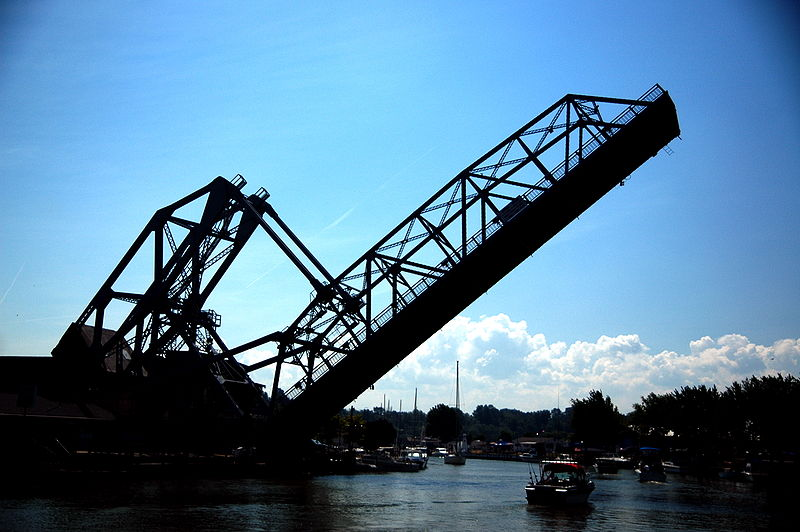
\includegraphics[width=2in]{./LawofSinesGraphics/AshBridge.jpg}}

\smallskip


Assume the bridge casts a shadow directly below itself the entire time it is being raised,\footnote{That is, the sun is directly overhead of the bridge and is shining for an entire two minutes... which never actually happens.} 

\begin{enumerate}

\item  Let $s$ denote the length of the shadow of the bridge on the water.  Show $s = 160 \cos(\theta)$. 
 
\smallskip

\item Assuming  the angle of elevation of the bridge changes at a constant rate, use the related rate law:\footnote{Theorem \ref{relatedratesaroc} in Section  \ref{RelatedRates}} $\frac{\Delta s}{\Delta t} = \frac{\Delta s}{\Delta \theta} \, \frac{\Delta \theta}{\Delta t}$   to help you find the rate of change of the shadow length with respect to time as $\theta$ increases from $30^{\circ}$ to $30.1^{\circ}$.  Remember to give units.


\end{enumerate}

\setcounter{HW}{\value{enumi}}
\end{enumerate}

\begin{enumerate}
\setcounter{enumi}{\value{HW}}

\item Prove that the Law of Sines holds when $\triangle ABC$ is a right triangle.

\item Discuss with your classmates why knowing only the three angles of a triangle is not enough to determine any of the sides.

\item Discuss with your classmates why the Law of Sines cannot be used to find the angles in the triangle when only the three sides are given.  Also discuss what happens if only two sides and the angle between them are given.  (Said another way, explain why the Law of Sines cannot be used in the SSS and SAS cases.)

\item Given $\alpha = 30^{\circ}$ and $b = 10$, choose four different values for $a$ so that 

\begin{enumerate}

\item the information yields no triangle
\item the information yields exactly one right triangle
\item the information yields two distinct triangles
\item the information yields exactly one obtuse triangle

\end{enumerate}

Explain why you cannot choose $a$ in such a way as to have $\alpha = 30^{\circ}$, $b = 10$ and your choice of $a$ yield only one triangle where that unique triangle has three acute angles.

\item Use the cases and diagrams in the proof of the Law of Sines (Theorem \ref{lawofsines}) to prove the area formulas given in Theorem \ref{areaformulasine}.  Why do those formulas yield square units when four quantities are being multiplied together?

\setcounter{HW}{\value{enumi}}

\end{enumerate}

\newpage

\subsection{Answers}

\begin{multicols}{2}

\begin{enumerate}

\item $\begin{array}{lll}
\alpha = 13^{\circ} & \beta = 17^{\circ} & \gamma = 150^{\circ} \\
a = 5 & b \approx 6.50 & c \approx 11.11 \end{array}$

\item $\begin{array}{lll}
\alpha = 73.2^{\circ} & \beta = 54.1^{\circ} & \gamma = 52.7^{\circ} \\
a = 117 & b \approx 99.00 & c \approx 97.22 \end{array}$

\setcounter{HW}{\value{enumi}}

\end{enumerate}

\end{multicols}

\begin{multicols}{2} 

\begin{enumerate}

\setcounter{enumi}{\value{HW}}

\item \begin{tabular}{l}
Information does not \\
produce a triangle \end{tabular}

\item $\begin{array}{lll}
\alpha = 95^{\circ} & \beta = 62^{\circ} & \gamma = 23^{\circ} \\
a = 33.33 & b \approx 29.54 & c \approx 13.07 \end{array}$

\setcounter{HW}{\value{enumi}}

\end{enumerate}

\end{multicols}

\begin{multicols}{2} 

\begin{enumerate}

\setcounter{enumi}{\value{HW}}

\item \begin{tabular}{l}
Information does not \\
produce a triangle \end{tabular}

\item $\begin{array}{lll}
\alpha = 117^{\circ} & \beta \approx 56.3^{\circ} & \gamma \approx 6.7^{\circ} \\
a = 45 & b = 42 & c \approx 5.89 \end{array}$

\setcounter{HW}{\value{enumi}}

\end{enumerate}

\end{multicols}

\begin{multicols}{2} 

\begin{enumerate}

\setcounter{enumi}{\value{HW}}

\item $\begin{array}{lll}
\alpha = 68.7^{\circ} & \beta \approx 76.9^{\circ} & \gamma \approx 34.4^{\circ} \\
a = 88 & b = 92 & c \approx 53.36 \end{array}$

$\begin{array}{lll}
\alpha = 68.7^{\circ} & \beta \approx 103.1^{\circ} & \gamma \approx 8.2^{\circ} \\
a = 88 & b = 92 & c \approx 13.47\end{array}$

\item $\begin{array}{lll}
\alpha = 42^{\circ} & \beta \approx 67.66^{\circ} & \gamma \approx 70.34^{\circ} \\
a = 17 & b = 23.5 & c \approx 23.93 \end{array}$

$\begin{array}{lll}
\alpha = 42^{\circ} & \beta \approx 112.34^{\circ} & \gamma \approx 25.66^{\circ} \\
a = 17 & b = 23.5 & c \approx 11.00 \end{array}$

\setcounter{HW}{\value{enumi}}

\end{enumerate}

\end{multicols}

\begin{multicols}{2} 

\begin{enumerate}

\setcounter{enumi}{\value{HW}}

\item \begin{tabular}{l}
Information does not \\
produce a triangle \end{tabular}

\item $\begin{array}{lll}
\alpha = 30^{\circ} & \beta = 90^{\circ} & \gamma = 60^{\circ} \\
a = 7 & b = 14 & c = 7\sqrt{3} \end{array}$

\setcounter{HW}{\value{enumi}}

\end{enumerate}

\end{multicols}

\begin{multicols}{2} 

\begin{enumerate}

\setcounter{enumi}{\value{HW}}

\item $\begin{array}{lll}
\alpha = 42^{\circ} & \beta \approx 23.78^{\circ} & \gamma \approx 114.22^{\circ} \\
a = 39 & b = 23.5 & c \approx 53.15 \end{array}$

\item $\begin{array}{lll}
\alpha = 53^{\circ} & \beta = 74^{\circ} & \gamma = 53^{\circ} \\
a = 28.01 & b \approx 33.71 & c = 28.01 \end{array}$

\setcounter{HW}{\value{enumi}}

\end{enumerate}

\end{multicols}

\begin{multicols}{2} 

\begin{enumerate}

\setcounter{enumi}{\value{HW}}

\item $\begin{array}{lll}
\alpha = 6^{\circ} & \beta \approx 169.43^{\circ} & \gamma \approx 4.57^{\circ} \\
a = 57 & b = 100 & c \approx 43.45 \end{array}$

$\begin{array}{lll}
\alpha = 6^{\circ} & \beta \approx 10.57^{\circ} & \gamma \approx 163.43^{\circ} \\
a = 57 & b = 100 & c \approx 155.51 \end{array}$

\item $\begin{array}{lll}
\alpha \approx 78.59^{\circ} & \beta \approx 26.81^{\circ} & \gamma = 74.6^{\circ} \\
a = 3.05 & b \approx 1.40 & c = 3 \end{array}$

$\begin{array}{lll}
\alpha \approx 101.41^{\circ} & \beta \approx 3.99^{\circ} & \gamma = 74.6^{\circ} \\
a = 3.05 & b \approx 0.217 & c = 3 \end{array}$

\setcounter{HW}{\value{enumi}}

\end{enumerate}

\end{multicols}

\begin{multicols}{2} 

\begin{enumerate}

\setcounter{enumi}{\value{HW}}

\item $\begin{array}{lll}
\alpha \approx 28.61^{\circ} & \beta = 102^{\circ} & \gamma \approx 49.39^{\circ} \\
a \approx 8.20 & b = 16.75 & c = 13 \end{array}$

\item \begin{tabular}{l}
Information does not \\
produce a triangle \end{tabular}

\setcounter{HW}{\value{enumi}}

\end{enumerate}

\end{multicols}

\begin{multicols}{2} 

\begin{enumerate}

\setcounter{enumi}{\value{HW}}

\item $\begin{array}{lll}
\alpha = 43^{\circ} & \beta = 102^{\circ} & \gamma = 35^{\circ} \\
a \approx 11.68 & b = 16.75 & c \approx 9.82 \end{array}$

\item $\begin{array}{lll}
\alpha = 66.92^{\circ} & \beta = 29.13^{\circ} & \gamma = 83.95^{\circ} \\
a \approx 593.69 & b = 314.15 & c \approx 641.75 \end{array}$

\setcounter{HW}{\value{enumi}}

\end{enumerate}

\end{multicols}

\begin{multicols}{2} 

\begin{enumerate}

\setcounter{enumi}{\value{HW}}

\item \begin{tabular}{l}
Information does not \\
produce a triangle \end{tabular}

\item $\begin{array}{lll}
\alpha = 50^{\circ} & \beta \approx 22.52^{\circ} & \gamma \approx 107.48^{\circ} \\
a = 25 & b = 12.5 & c \approx 31.13 \end{array}$

\setcounter{HW}{\value{enumi}}

\end{enumerate}

\end{multicols}

\begin{enumerate}

\setcounter{enumi}{\value{HW}}

\item The area of the triangle from Exercise \ref{firstlawofsines} is about 8.1 square units.\\
The area of the triangle from Exercise \ref{secondarea} is about 377.1 square units.\\
The area of the triangle from Exercise \ref{lastlawofsines} is about 149 square units.

\item $\arctan\left(\frac{7}{100}\right) \approx 0.699$ radians, which is equivalent to $4.004^{\circ}$
\item About 17\%
\item About 53 feet

\pagebreak

\item \begin{multicols}{4} \begin{enumerate}

\item $\theta = 180^{\circ}$
\item $\theta = 353^{\circ}$
\item $\theta = 84.5^{\circ}$
\item $\theta = 270^{\circ}$

\setcounter{HWindent}{\value{enumii}}

\end{enumerate}

\end{multicols}

\begin{multicols}{4} 

\begin{enumerate}

\setcounter{enumii}{\value{HWindent}}

\item $\theta = 121.25^{\circ}$
\item $\theta = 197^{\circ} 18' 48''$
\item $\theta = 45^{\circ}$
\item $\theta = 225^{\circ}$

\end{enumerate}

\end{multicols}

\item  The Colonel is about 3193 feet from the campfire. \\
Sarge is about 2525 feet to the campfire.

\item The distance from the Muffin Ridge Observatory to Sasquach Point is about 7.12 miles.\\
The distance from Sasquatch Point to the Chupacabra Trailhead is about 2.46 miles.

\item  The SS Bigfoot is about 4.1 miles from the flare. \\
The HMS Sasquatch is about 2.9 miles from the flare.

\item  Jeff is about 371 feet from the nest.

\item  She is about 3.02 miles from the lodge

\item  The boat is about 25.1 miles from the second tower.

\item  The UFO is hovering about 9539 feet above the ground.

\item The gargoyle is about 44 feet from the observer on the upper floor. \\
The gargoyle is about 27 feet from the observer on the lower floor. \\
The gargoyle is about 25 feet from the other building.

\setcounter{HW}{\value{enumi}}
\end{enumerate}

\begin{enumerate}
\setcounter{enumi}{\value{HW}}
\item \begin{enumerate} \addtocounter{enumii}{1}

\item  $\frac{\Delta h}{\Delta t}$ is given as a constant $6 \, \frac{\text{ft}}{\text{s}}$. $\frac{\Delta h}{\Delta \theta} = \frac{h(60.1) - h(60)}{0.1} \approx 0.348 \, \frac{\text{ft}}{\text{degree,  } \,  \circ}$.  

\smallskip

Hence, $\frac{\Delta \theta}{\Delta t} = \frac{ 6 \, \frac{\text{ft}}{\text{s}}   }{ 0.348 \, \frac{\text{ft}}{\text{degree,  } \, \circ}} \approx 17.215 \, \frac{ \text{degree,  } \, \circ}{s}$.  

\smallskip

The angle of elevation is increasing at an average rate of $17.215$ degrees  per second.  

\smallskip

\textbf{WARNING:} For (good) reasons you'll explore more deeply in Calculus, you'll usually stick with radians when the Calculus version of this problem rolls around \ldots  

\end{enumerate}


\item  \begin{enumerate} \addtocounter{enumii}{1}

\item   $\frac{\Delta s}{\Delta \theta} = \frac{s(30.1) - s(30)}{0.1} \approx -1.398 \, \frac{\text{ft}}{\text{degree} \,  \circ}$.  

\smallskip

We are told to assume $\frac{\Delta \theta }{\Delta t}$ is a constant, so $\frac{\Delta s}{\Delta t} = \frac{45^{\circ}}{2 \, \text{minutes}} = 22.5 \, \frac{\text{degree,  } \, \circ}{\text{min}}$.

\smallskip

We get:  $\frac{\Delta s}{\Delta t} = \frac{\Delta s}{\Delta \theta} \, \frac{\Delta \theta }{\Delta t} \approx \left(-1.398 \, \frac{\text{ft}}{\text{degree,  } \,  \circ} \right) \left(  22.5 \, \frac{\text{degree,  } \, \circ}{\text{min}} \right) \approx -31.436 \, \frac{\text{ft}}{\text{min}}$.

\smallskip

This means the shadow is receding at a rate of approximately 31.436 feet per minute.

\smallskip

\textbf{WARNING:} For (good) reasons you'll explore more deeply in Calculus, you'll usually stick with radians when the Calculus version of this problem rolls around \ldots  

\end{enumerate}


\setcounter{HW}{\value{enumi}}
\end{enumerate}




\end{document}


\closegraphsfile

\end{document}
